\vspace{-1cm}
\begin{wrapfigure}[13]{r}{5cm}
  \centering
  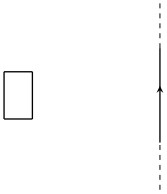
\includegraphics[width=0.25\textwidth]{Figures/Fig 4.jpg}
  \begin{center}
    \figurename{ 4}
  \end{center}
\end{wrapfigure}

\noindent Một khung dây cứng, mảnh hình chữ nhật có thể di chuyển trên bề mặt nằm ngang và nhẵn, trên bề mặt có gắn cố định một sợi dây thẳng, mảnh, và dài vô hạn như hình 4. Ban đầu, cường độ dòng điện trong dây dẫn và khung dây bằng không. Khung dây nằm yên ở vị trí sao cho một cặp cạnh của nó song song với dây dẫn và khoảng cách giữa dây dẫn và cạnh gần nhất của khung dây rất lớn so với kích thước của khung. Sau đó, cường độ dòng điện trong dây dẫn được tăng lên đến một giá trị cực đại nào đó và được giữ không đổi ở giá trị này. Giả sử thời gian thực hiện là rất ngắn, đủ để bỏ qua chuyển động của khung dây trong quá trình này. Khi cường độ dòng điện trong dây dẫn đạt giá trị cực đại, vận tốc của khung dây là $v_{0}$. Bỏ qua độ tự cảm của khung và xem như điện trở của khung không đổi. Biết rằng sau một khoảng thời gian rất dài kể từ khi cường độ dòng điện trong dây dẫn đạt giá trị cực đại, vận tốc của khung không đổi và bằng $v_{1}$. Tìm $v_{1}$.\\